%%%%%%%%%%%%%%%%%%%%%%%%%%%%%%%%%%%%%%%%%%%%%%%%%%%%%%%%%%%%%%%%%%%%
%% I, the copyright holder of this work, release this work into the
%% public domain. This applies worldwide. In some countries this may
%% not be legally possible; if so: I grant anyone the right to use
%% this work for any purpose, without any conditions, unless such
%% conditions are required by law.
%%%%%%%%%%%%%%%%%%%%%%%%%%%%%%%%%%%%%%%%%%%%%%%%%%%%%%%%%%%%%%%%%%%%

\documentclass[
  digital, %% This option enables the default options for the
           %% digital version of a document. Replace with `printed`
           %% to enable the default options for the printed version
           %% of a document.
  twoside, %% This option enables double-sided typesetting. Use at
           %% least 120 g/m² paper to prevent show-through. Replace
           %% with `oneside` to use one-sided typesetting; use only
           %% if you don’t have access to a double-sided printer,
           %% or if one-sided typesetting is a formal requirement
           %% at your faculty.
  table,   %% This option causes the coloring of tables. Replace
           %% with `notable` to restore plain LaTeX tables.
  nolof,     %% This option prints the List of Figures. Replace with
           %% `nolof` to hide the List of Figures.
  nolot,     %% This option prints the List of Tables. Replace with
           %% `nolot` to hide the List of Tables.
  %% More options are listed in the user guide at
  %% <http://mirrors.ctan.org/macros/latex/contrib/fithesis/guide/mu/fi.pdf>.
]{fithesis3}
%% The following section sets up the locales used in the thesis.
\usepackage[resetfonts]{cmap} %% We need to load the T2A font encoding
\usepackage[T1,T2A]{fontenc}  %% to use the Cyrillic fonts with Russian texts.
\usepackage[
  main=english, %% By using `czech` or `slovak` as the main locale
                %% instead of `english`, you can typeset the thesis
                %% in either Czech or Slovak, respectively.
  english, german, russian, czech, slovak %% The additional keys allow
]{babel}        %% foreign texts to be typeset as follows:
%%
%%   \begin{otherlanguage}{german}  ... \end{otherlanguage}
%%   \begin{otherlanguage}{russian} ... \end{otherlanguage}
%%   \begin{otherlanguage}{czech}   ... \end{otherlanguage}
%%   \begin{otherlanguage}{slovak}  ... \end{otherlanguage}
%%
%% For non-Latin scripts, it may be necessary to load additional
%% fonts:
\usepackage{paratype}
\def\textrussian#1{{\usefont{T2A}{PTSerif-TLF}{m}{rm}#1}}
%%
%% The following section sets up the metadata of the thesis.
\thesissetup{
    date          = \the\year/\the\month/\the\day,
    university    = mu,
    faculty       = fi,
    type          = mgr,
    author        = Bc. Andrej Staruch,
    gender        = m,
    advisor       = {RNDr. Marek Kumpošt, Ph.D.},
    title         = {Phishing-detection application},
    TeXtitle      = {Phishing-detection application},
    keywords      = {phishing, anti-spam, application},
    TeXkeywords   = {phishing, anti-spam, application},
    abstract      = {The goal of this master's thesis is to develop and implement an application, which will recognize potential risk for a given URL from web traffic based on extendable series of individual tests. The result of weighted tests is 'phishing score' and one of three actions for an URL: bypass, warn and block. The source for  tests should be this following work: https://is.muni.cz/auth/th/dyi2v/Diplomova\_prace.pdf
    
    },
    thanks        = {These are the acknowledgements for my thesis, Mgr. Karol Kubanda, učo 143339 (konzultant) },
    bib           = example.bib,
}
\usepackage{makeidx}      %% The `makeidx` package contains
\makeindex                %% helper commands for index typesetting.
%% These additional packages are used within the document:
\usepackage{paralist} %% Compact list environments
\usepackage{amsmath}  %% Mathematics
\usepackage{amsthm}
\usepackage{amsfonts}
\usepackage{url}      %% Hyperlinks
\usepackage{markdown} %% Lightweight markup
\usepackage{listings} %% Source code highlighting
\lstset{
  basicstyle      = \ttfamily,%
  identifierstyle = \color{black},%
  keywordstyle    = \color{blue},%
  keywordstyle    = {[2]\color{cyan}},%
  keywordstyle    = {[3]\color{olive}},%
  stringstyle     = \color{teal},%
  commentstyle    = \itshape\color{magenta}}
\usepackage{floatrow} %% Putting captions above tables
\floatsetup[table]{capposition=top}
\begin{document}
\chapter{Introduction}

In today's world, the threat of a cyber attack can't be ignored. There are a plethora of companies that try to protect their customers from potential damage, such as getting infected by a virus, getting ransomware or malware or protect their business intelligence.

This thesis is concerned with another part of the cyber crime called phishing. Phishing is a social engineering attack to obtain sensitive information such as usernames, passwords, credit card details, bank account credentials for malicious reasons. Because of a large attack vector, there isn't a reliable way or a tool to prevent such an attack consistently in every sector.

This thesis will review several ways to detect a phishing attack, implement some of them and test them in the production environment with an association with a Trusted Network Solutions company. The final software could be easily used with another proxy or tool.

The word phishing is originated from the word fishing - attackers fishes on their victims. Phishers use a number of techniques to trick their possible victims: having a fake clone site like the original one with forms so a user will enter credentials to their site, or sending e-mails with messages to send money to some address.

The total number of phish detected in 2Q 2018 was 233,040, compared to 263,538 in 1Q 2018. These totals exceed the 180,577 observed in 4Q 2017 and the 190,942 seen in 3Q 2017 [1].

TODO: preložiť, upraviť, toto je len nástrel a bude sa to meniť ako celá úvodná kapitola počas celej doby trvania práce. Dokým sa rozpíšem a nájdem systém tak tieto omáčky budem písať radšej v slovenčine.

Nezisková organizácia APWG, ktorá ma za cieľ zjednotiť obranu voči cyberútokom, pravidelne vytvára štatistiky o aktuálnych trendoch a počtoch phishing útokov. Na číslach za uplynulý pol rok je vidno, že sa celkový počet pohybuje v podobnej rovine:

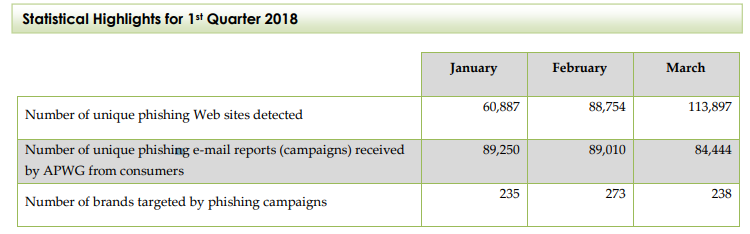
\includegraphics[width=1.0\textwidth]{images/2018q1.png}
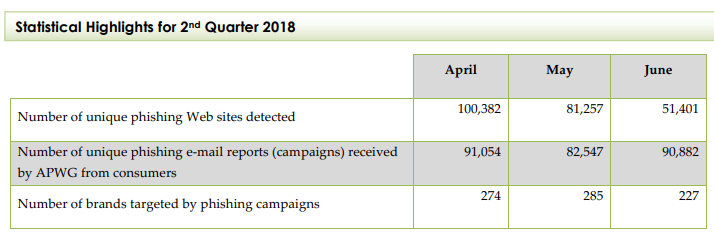
\includegraphics[width=1.0\textwidth]{images/2018q2.png}

Počet jednotlivých stránok má rôzne výkyvy, zatiaľ čo počet e-mailov sa postupne zvyšuje. Na základe analýz životnosti jednotlivých phishingových kampaní sa zistilo, že priemerná živostnosť je okolo 12 hodín [2]. Táto skutočnosť výrazne ovplyvňuje schopnosť automaticky detekovať phishingový útok (doplniť rozumný dôvod, citáciu).

Rozdelenie ako sa môže phishingový útok detekovať, by sa dalo nasledovne kategorizovať:
\begin{enumerate}
    \item detekcia na základe blacklistov
    \item detekcia na základe heuristiky
    \item detekcia na základe vizuálnej podobnosti
    \item detekcia na základe histórie a vlastnosti stránky
\end{enumerate}

Detekcia na základe blacklistov je najjednoduhším mechanizmom - zašleme request na API z niektorých poskytovateľov, poprípade sa pozrieme do lokálnej databázy. Nevýhoda týchto databáz je ich neaktuálnosť, pretože aby sa adresa objavila v zozname, tak musí prejsť procesom schválenia. Takisto tieto zoznamy neposkytujú ocharnu proti novým útokom a keď že trvácnosť stránok sa pohybuje v rádoch hodín, nie je toto dostatočná ochrana a mala by byť kombinovaná s niektorou inou.

Detekcií na základe heuristiky môže byť veľké množstvo, v tejto práci sa budeme venovať najmä na zadávanie pravidiel na to, ako vyzerá phishingová URL a priraďovaniu hodnôt pre dané pravidlá. Jedná sa napríklad o:
\begin{enumerate}
    \item dĺžka URL
    \item špeciálne znaky
    \item hĺbka zanorenia
    \item použitie IP adresy namiesto hostname
\end{enumerate}


TODO: spomenút výskum čo vyšiel v oktobér 2018 ohľadom toho že 35 percent phishingových stránok ma https a že tento trend ma stúpajúci charakter.

TODO: spomenúť význam tejto práce, že sa ešte nenachádza komplexné riešenie pre integráciu do proxy pre lokálny trh

TODO: poriadne odcitovať všetky horné poznatky aby to nebol kompilát.

TODO: Pridať odstavec o detekcii na základe vizuálnej podobnosti.

TODO: pridať odstavec ohľadom toho, že táto práca bude slúžiť ako ochrana pre užívateľov za proxy.

\chapter{These are}
\section{the available}
\subsection{sectioning}
\subsubsection{commands.}
\paragraph{Paragraphs and}
\subparagraph{subparagraphs are available as well.}
Inside the text, you can also use unnumbered lists,


\chapter{Using lightweight markup}
\shorthandoff{-}
\begin{markdown*}{%
  hybrid,
  definitionLists,
  footnotes,
  inlineFootnotes,
  hashEnumerators,
  fencedCode,
  citations,
  citationNbsps,
}

If you decide that \LaTeX{} is too wordy for some parts of your
document, there are [packages](https://www.ctan.org/pkg/markdown
"Markdown") that allow you to use more lightweight markup next
to it.

 ![logo](fithesis/logo/mu/fithesis-base.pdf "The logo of the
  Masaryk University")

This is a bullet list. Unlike numbered lists, bulleted lists
contain an **unordered** set of bullet points. When a bullet point
contains multiple paragraphs, the list is typeset as follows:

  * The first item of a bullet list

    that spans several paragraphs,
  * the second item of a bullet list,
  * the third item of a bullet list.

When none of the bullet points contains multiple paragraphs, the
list has a more compact form:

  * The first item of a bullet list,
  * the second item of a bullet list,
  * the third item of a bullet list.

Unlike a bulleted list, a numbered list implies chronology or
ordering of the bullet points. When a bullet point
contains multiple paragraphs, the list is typeset as follows:

  1. The first item of an ordered list

     that spans several paragraphs,
  2. the second item of an ordered list,
  3. the third item of an ordered list.
  #. If you are feeling lazy,
  #. you can use hash enumerators as well.

When none of the bullet points contains multiple paragraphs, the
list has a more compact form:

  6. The first item of an ordered list,
  7. the second item of an ordered list,
  8. the third item of an ordered list.

Definition lists are used to provide definitions of terms. When
a definition contains multiple paragraphs, the list is typeset
as follows:

Term 1

:   Definition 1

*Term 2*

:   Definition 2

        Some code, part of Definition 2

    Third paragraph of Definition 2.

When none of the bullet points contains multiple paragraphs, the
list has a more compact form:

Term 1
:   Definition 1
*Term 2*
:   Definition 2

Block quotations are used to include an excerpt from an external
document in way that visually clearly separates the excerpt from
the rest of the work:

> This is the first level of quoting.
>
> > This is nested blockquote.
>
> Back to the first level.

Footnotes are used to include additional information to the
document that are not necessary for the understanding of the main
text. Here is a footnote reference^[Here is the footnote.] and
another.[^longnote]

[^longnote]: Here's one with multiple blocks.

    Subsequent paragraphs are indented to show that they
belong to the previous footnote.

        Some code

    The whole paragraph can be indented, or just the first
    line.  In this way, multi-paragraph footnotes work like
    multi-paragraph list items.

Citations are used to provide bibliographical references to other
documents. This is a regular citation~[@borgman03, p. 123]. This is
an in-text citation: @borgman03\. You can also cite several authors
at once using both regular~[see @borgman03, p. 123; @greenberg98,
sec.  3.2; and @thanh01] and in-text citations: @borgman03 [p.123;
@greenberg98, sec. 3.2; @thanh01].

Code blocks are used to include source code listings into the
document:

    #include <stdio.h>
    #include <unistd.h>
    #include <sys/types.h>
    #include <sys/wait.h>
    // This is a comment
    int main(int argc, char **argv)
    {
        while (--c > 1 && !fork());
        sleep(c = atoi(v[c]));
        printf("%d\n", c);
        wait(0);
        return 0;
    }

There is an alternative syntax for code blocks that allows you to
specify additional information, such as the language of the source
code. This information can be used for syntax highlighting:

``` sh
#!/bin/sh
fac() {
  if [ "$1" -leq 1 ]; then
    echo 1
  else
    echo $(("$1" * fac $(("$1" - 1))))
  fi
}
``````````````

~~~~~~ Ruby
# Here's a way to empty an array.
joe = [ 'eggs.', 'some', 'break', 'to', 'Have' ]
print(joe.pop, " ") while joe.size > 0
print "\n"
~~~~~~

\end{markdown*}
\shorthandon{-}

\chapter{Inserting the bibliography}
After linking a bibliography data\-base files to the document using
the \verb"\"\texttt{thesis\discretionary{-}{}{}setup\{bib\discretionary{=}{=}{=}%
\{\textit{file1},\textit{file2},\,\ldots\,\}\}} command, you can
start citing the entries. This is just dummy text
\parencite{rrphish} lightly sprinkled with citations
\parencite[p.~123]{greenberg98}. Several sources can be cited at
once: \cite{borgman03,greenberg98,thanh01}.
\citetitle{greenberg98} was written by \citeauthor{greenberg98} in
\citeyear{greenberg98}. We can also produce \textcite{greenberg98}%
\ or %% Let us define a compound command:
\def\citeauthoryear#1{(\textcite{#1},~\citeyear{#1})}%
\citeauthoryear{greenberg98}%
. The full bibliographic citation is:
\emph{\fullcite{greenberg98}}. We can easily insert a bibliographic
citation into the footnote\footfullcite{greenberg98}.

The \verb"\nocite" command will not generate any
output\nocite{muni}, but it will insert its arguments into
the bibliography. The \verb"\nocite{*}" command will insert all the
records in the bibliography database file into the bibliography.
Try uncommenting the command
%% \nocite{*}
and watch the bibliography section come apart at the seams.

When typesetting the document for the first time, citing a
\texttt{work} will expand to [\textbf{work}] and the
\verb"\printbibliography" command will produce no output. It is now
necessary to generate the bibliography by running \texttt{biber
\jobname.bcf} from the command line and then by typesetting the
document again twice. During the first run, the bibliography
section and the citations will be typeset, and in the second run,
the bibliography section will appear in the table of contents.

The \texttt{biber} command needs to be executed from within the
directory, where the \LaTeX\ source file is located. In Windows,
the command line can be opened in a directory by holding down the
\textsf{Shift} key and by clicking the right mouse button while
hovering the cursor over a directory.  Select the \textsf{Open
Command Window Here} option in the context menu that opens shortly
afterwards.

With online services -- such as Overleaf -- or when using an
automatic tool -- such as \LaTeX MK -- all commands are executed
automatically. When you omit the \verb"\printbibliography" command,
its location will be decided by the template.

  \printbibliography[heading=bibintoc] %% Print the bibliography.


\end{document}
